\chapter{Theory}

\section{Previous work}

The first major work in the area of generating images was done by Goodfellow~{\em et al.}~\cite{origgan} by introduction of Generative Adversarial Networks. Since then many variants improving on the original paper emerged focusing on different tasks.

In the area of image translation, Isola~{\em et al.}~\cite{pix2pix} introduced pixel-wise loss in order to generate visually appealing yet constrained images. Similar approach was taken by Shrivastava~{\em et al.}~\cite{historypool}, with their SimGAN which introduced self-regularization loss to constrain generation process within the desired direction and were able to solve the generative task within semi-supervised settings.

Later on Isola~{\em et al.} introduced CycleGAN~\cite{cyclegan} with the cycle consistency loss in order to solve the image translation task without paired correspondences. However, all of the recent work was done only on regular images. As far as we know we have not find any published work in the area of generating or translating depth data from LiDAR sensors.

\section{Used neural networks} \label{nets}

The neural networks (sometimes also called artificial neural networks or ANNs) are a powerful tool of today's machine learning. The main component is an {\em artificial neuron}, a computational unit which takes an input and computes a predefined (usually linear) function with its internal parameters. This output is then optionally fed through (usually nonlinear) {\em activation function} to introduce nonlinearities in the output. The artificial neurons can be stacked next to each other to form layers, and if we connect multiple layers together, we have a neural network. We can think of the neural network as a nonlinear transformation function with multiple internal parameters.

The process of training the neural network to give the output we desire then consists of feeding the input data into the network and evaluating the performance by the {\em loss function}, which computes a real-valued number associating the actual output of the network with a notion of a ``badness'' in comparison with the expected output. This loss function could be for example a norm of a difference between the output of the network and the output given by a human in the case of image labeling or it could be more complex function altogether. The loss function is then minimized with respect to the internal parameters of the neural network by gradient descent algorithm. The most used gradient descent algorithm is a stochastic descent and its variants such as Adam~\cite{adam} or Adagrad~\cite{adagrad}.

If the loss function is well defined over the problem set, then the network will give the desired results at the global minimum of the loss function. However, since this function is a function of the {\em parameters} of the network, it is generally not convex and highly dimensional, and therefore it is hard to reach the global minimum. LeCun~\cite{efbackprop} gave numerous tricks to improve the likelihood of finding a good enough local minimum.

The neural layers we introduced above are usually called {\em fully connected} because all the outputs from one layer are connected to all the neurons from the next layer. This was one of the first formulations of artificial neural networks~\cite{orignet}. However, these fully connected layers are not well suited for computer vision applications, since we would like to have the same response to the particular object in the image regardless of its position or orientation. To overcome this issue, the {\em convolutional} layers~\cite{convnet}, which perform a mathematical operation of convolution over the input, were introduced. Quite often these convolutional layers are followed by the fully connected layers at the end of the network.

A recently proposed residual block~\cite{resnet} also plays an important role in current state of the art architectures. The paper proposes to instead of learning the mapping $\bm{y} = f(\bm{x})$, it is easier to learn the mapping $h(\cdot)$ from equation $\bm{y} = h(\bm{x}) + \bm{x}$. The reasoning for this reformulation is that if it is needed to learn mapping close to identity it is much easier to learn it in this settings. It was shown by the original paper that they were able to reduce the sizes of the well-performing architectures while still maintaining or improving their accuracy. The only drawback of this residual block is that it cannot change the size of the input.

\subsection{Generative adversarial network (GAN)}

A generative adversarial network is a concept by Ian Goodfellow~\cite{origgan} aimed at learning to generate a sample from a particular distribution. The main goal is to train a {\em generator} network to produce samples from the target distribution given a sample from some noise distribution. In order to achieve this, a second network called {\em discriminator} is introduced, and its main goal is to distinguish between the samples from the real target distribution and the ``fake'' samples produced by the generator network given a noise sample. If the whole setup is modeled in such a way that the trained discriminator outputs a scalar assigning a probability of the sample coming from the target distribution, the generator is then trying to produce the samples that are convincing enough to the discriminator so that discriminator's output for the generated samples is as close to 1 as possible. This setup was originally formulated within the maximum log-likelihood estimation setup. It could be seen as a two-player minimax game with the value function $V(G, D)$ shown in equation~\ref{gangame}, where $G$ and $D$ are generator and discriminator functions respectively, $p_{target}$ is a target distribution and $p_{noise}$ is a noise distribution that is usually chosen as a uniform, however it could be any other source of noise data.

\begin{equation}
\min_G \max_D V(G, D) = \EX_{\bm{x}\sim p_{target}}[\log D(\bm{x})] + \EX_{\bm{z}\sim p_{noise}} [\log(1 - D(G(\bm{z})))]
\label{gangame}
\end{equation}

This formulation immediately yields loss functions for the generator (equation \ref{ganlossg}) and discriminator (equation \ref{ganlossd}) where $\bm{x}$ are the samples from the target distribution that we present to the networks during the learning and $\bm{z}$ is a noise sampled at each iteration of the training algorithm.

\begin{equation}
\loss_G = \log(1 - D(G(\bm{z})))
\label{ganlossg}
\end{equation}

\begin{equation}
\loss_D = - (\log D(\bm{x}) + \log(1 - D(G(\bm{z}))))
\label{ganlossd}
\end{equation}

It was theoretically shown~\cite{origgan} that in the case of generator and discriminator having enough capacity this setup allows to train the generator to be able to generate samples indistinguishable from the samples from $p_{target}$. However this is not easily achievable in practice. One of the main problems is that generator usually does not have an infinite capacity. More problems stem from the fact that the original loss function (equation \ref{ganlossg}) for the generator does not provide strong enough gradients early in the process of training, therefore a new loss function with the same theoretical properties, but stronger gradients was introduced as shown in the equation \ref{ganlossgg}.

\begin{equation}
\loss_G = -\log(D(G(\bm{z})))
\label{ganlossgg}
\end{equation}

In practice, we are trying to find the Nash equilibrium~\cite{nash} of a highly dimensional, non-convex function and while we can obtain gradients for this function using training samples, there is no known algorithm to solve this game exactly~\cite{improvedgan}. To overcome this obstacle, it is recommended~\cite{origgan} to alternate between training step of the generator and the discriminator on the same data with discriminator being trained first. It is helpful for the training process to train discriminator near its optimum before updating generator and to achieve this, it might be necessary to train discriminator more than once for one batch of samples.

Another problem that could very easily occur is a {\em mode collapse} of the generator -- a point, where generator does not use its full potential and generates a fixed point for multiple inputs keeping discriminator in the dark. Since the generator receives its gradients from the discriminator and discriminator cannot give any useful information anymore, the generator will not be updated in any sensible direction past the point where the mode collapse occurred. After the mode collapse, it does not make any sense to train the affected networks anymore.

\subsection{GAN variants}

Since the inception of GANs, many variants emerged trying to overcome some of the issues outlined in the previous subsection. According to DeepHunt~\cite{deephunt}, there were 354 papers proposing a variation of GAN as of 10\textsuperscript{th} May 2018. Most of these improvements revolve around redefining the loss functions and introducing various tricks to achieve better training stability.

In the following subsections will be shortly described some of these variants with their particular improvements and differences from the original GAN.

\subsubsection{DCGAN -- Deep Convolutional GAN}
DCGAN~\cite{dcgan} is not a variant of GAN per se, as it mostly involves guidelines for stable training of GAN where discriminator and generator consist of multiple convolutional layers. The said guidelines can be briefly summarized as:
\begin{itemize}
\item Use strided convolution and deconvolution instead of pooling layers. The reasoning behind this is to allow the networks to find their own representations of up-sampling and down-sampling operations.
\item Use batch normalization~\cite{batchnorm} everywhere applicable (i.e. in every layer except the last one). This allows to normalize the gradients for every layer according to the batch.
\item Do not use fully connected layers that are not the direct output of the discriminator. If there are hidden fully connected layers, then the model stability might improve, however it reduces convergence speed of the training process.
\item Use ReLU~\cite{relu} activation for generator's layers except the last layer using hyperbolic tangent. It was observed, that ReLU helps convergence speed of the training process the most.
\item Use LeakyReLU~\cite{leakyrelu} activation for discriminator's layers. This seems to be especially helpful in higher resolution settings.
\item Use Adam~\cite{adam} optimizer with {\em different} hyperparameters than the usual default. Especially necessary is to lower the learning rate and momentum terms.
\end{itemize}

\subsubsection{LSGAN -- Least Squares GAN}
The main idea behind LSGAN~\cite{lsgan} is not to use maximum log-likelihood framework, but to use least squares instead. The formulation of the generator and discriminator loss functions can be then seen in equations \ref{lsganlossg} and \ref{lsganlossd}, where $a$, $b$ and $c$ are target values of the discriminator that we are aiming for. In most applications, $c = a = 1$ (or 0.9 to introduce label smoothing, as proposed by~\cite{improvedgan,smooth}) and $b = 0$.

\begin{equation}
\loss_G = \frac{1}{2}(D(G(\bm{z})) - c)^2
\label{lsganlossg}
\end{equation}

\begin{equation}
\loss_D = \frac{1}{2}(D(\bm{x}) - a)^2 + \frac{1}{2}(D(G(\bm{z})) - b)^2
\label{lsganlossd}
\end{equation}

The reasoning for this reformulation of the loss functions is mostly to provide better gradients and to move the generated samples closer to the decision boundary. In traditional GAN, samples that pass the decision boundary do not provide strong enough gradients and do not contribute to the learning process. However with the LSGAN, there is only one flat point of the loss functions without strong gradients.

\subsubsection{WGAN and WGAN-GP -- Wasserstein GAN (with gradient penalty)}

One of the ideas of the original GANs we have not talked about before is minimizing some metric between the generated and the target distributions. This metric is usually well defined by the respective loss function and for original formulation of GAN it is Kullback-Leibler divergence~\cite{kullback} and for LSGAN it is Pearson $\chi^2$ divergence~\cite{pearson}.

WGAN~\cite{wgan} was introduced to minimize Wasserstein-1 distance~\cite{wasser}, also known as Earth-Mover. This definition yields following loss functions as seen on equations \ref{wganlossg} and \ref{wganlossd}.

\begin{equation}
\loss_G = -D(G(\bm{z}))
\label{wganlossg}
\end{equation}

\begin{equation}
\loss_D = D(G(\bm{x})) - D(\bm{z})
\label{wganlossd}
\end{equation}

However, to enforce a Wasserstein-1 distance, it is necessary to satisfy the condition that function $D$ is K-Lipshitz continuous for any given K. This is not easy to achieve and the method used in the original paper was weight clipping to a tight bounding box after each update. It is worth noting the authors admit that this solution is impractical and obviously wrong, however they could not think of a better solution at the time.

The reformulation of WGAN called WGAN-GP~\cite{wgan-gp} emerged soon after and introduced less drastic way to enforce K-Lipshitz continuity. The discriminator's loss function would receive an additional term called gradient penalty forcing the gradients of the function to be ``approximately 1 almost everywhere''. This gradient penalty removes the need for the weight clipping in the original paper and it is shown in equation \ref{wgangplossgdp}, where $\bm{\tilde{x}} = \epsilon\bm{x} + (1 - \epsilon)G(\bm{z})$ and $\epsilon$ is a uniform random number from the range [0; 1].

\begin{equation}
\loss_{GP} = (\norm{\nabla_{\bm{\tilde{x}}}D(\bm{\tilde{x}})}_2 - 1)^2
\label{wgangplossgdp}
\end{equation}

It is now even more critical than in the original formulation of GAN to train the discriminator to almost optimum. This stems for the fact that better discriminator yields much stronger gradients than poorly trained one.

Authors of WGAN-GP showed, that the gradient penalty is superior to the weight clipping since the original WGAN exhibited either vanishing or exploding gradients quite often. To demonstrate higher stability, WGAN-GP authors trained many architectures with this criterion on ImageNet~\cite{imagenet} dataset and measured the Inception score~\cite{improvedgan} (score based on ability to produce samples from different ImageNet classes with high classification rate by Inception network~\cite{inception}) achieved by the network. It was shown~\cite{wgan-gp}, that many more architectures were able to obtain high Inception score when trained by WGAN-GP loss functions instead of original GAN loss functions.

Quite an important thing to note is the fact, that WGAN-GP {\em cannot} use popular Batch normalization~\cite{batchnorm} layers as it alters the gradients of the layers and makes the gradient penalty useless. The recommendation by the article authors is to use Layer normalization~\cite{layernorm} layers instead. It is also beneficial to widen the range of the discriminator function to [-1; 1] (as opposed to [0; 1] in the original GAN) and to achieve this, it suffices to only change the activation function of the last layer of the discriminator to hyperbolic tangent.

\subsection{SimGAN}

SimGAN~\cite{historypool} is GAN variant aiming to learn a {\em refinement} of simulated data to make them look realistic enough. The paper called the generator network with the name {\em refiner} to emphasize the fact, that it received simulated data (instead of noise) on the input. The paper introduced three important concepts in the field of GANs. The first one is {\em local} adversarial loss -- this idea means, that the discriminator should not produce only scalar output, but a response map, where each part of this map corresponds to the particular patch of the evaluated image. The reasoning behind this is to allow patches with not so dominant features to contribute to the loss of the discriminator and by extension of the refiner as well.

Second key idea is adding a so-called {\em self-regularization} term to the refiner's loss function. This term can be seen in equation \ref{simganself}, where $\bm{x}$ is a sample from simulated data (refiner's input), $\bm{\tilde{x}}$ is a refined sample (refiner's output), $\lambda_{reg}$ is a relative weight given to the importance of this loss term and $\psi$ is a feature mapping from image space to the feature space. This feature mapping could be any function with important properties (such as classification of the data), or it could be simple identity and then the $\loss_{reg}$ would become pixel-wise distance.

\begin{equation}
\loss_{reg} = \lambda_{reg}\norm{\psi({\bm{x}}) - \psi({\bm{\tilde{x}}})}_1
\label{simganself}
\end{equation}

This self-regularization term allows to teach the refiner to keep the most important information of the image during the refinement process.

Third key idea is to introduce memory for the discriminator's learning process. The discriminator should be unable to forget about the images it has seen an epoch ago. In order to facilitate this memory, a history buffer which keeps the refined samples is introduced. When performing single optimization step on discriminator weights, approximately half of the used batch is replaced with the samples from this history buffer. To be able to limit the buffer size, after performing the training step, half of the samples from the batch is randomly selected and random samples in the history buffer are replaced by this selection.

\subsection{CycleGAN} \label{cyclegan}

CycleGAN~\cite{cyclegan} is a concept aiming to match two different distributions by the means of GANs. The core idea is to have {\em two} GANs trained simultaneously with one generator learning the mapping from the first distribution to the second and the other generator learning the reverse mapping. To enforce this reverse mapping, new term called {\em cycle consistency loss} is added to the loss function of the generators. This loss term can be seen in the equation \ref{cycleloss}, where $p_X, p_Y$ are the distributions between which we try to find a mapping $\bm{x}\sim p_X$, $\bm{y}\sim p_Y$, $G_{X\rightarrow Y}$ is a generator mapping from $p_X$ to $p_Y$, $G_{X\rightarrow Y}$ is a generator mapping from $p_Y$ to $p_X$ and $\lambda_{cyc}$ is a relative weight given to the importance of this loss term.

\begin{equation}
\loss_{cyc} = \lambda_{cyc}(\norm{G_{Y\rightarrow X}(G_{X\rightarrow Y}(\bm{x})) - \bm{x}}_1 + \norm{G_{X\rightarrow Y}(G_{Y\rightarrow X}(\bm{y})) - \bm{y}}_1)
\label{cycleloss}
\end{equation}

This approach of training two GANs simultaneously can give us mapping between these two distributions {\em without} having a pair-to-pair correspondences. It is important to note that even though this closely relates to the style transfer problem, the resulting mappings should work in both directions which is usually not the case with more common approaches~\cite{artstyle} to the style transfer. Since this seems like an approach that could help us model the mapping between real-life and in-game data of the cars' sensors, we decided to use CycleGAN as a basis for our experiments using various underlying architectures of GANs.

The CycleGAN does not concern itself with the particular type of GAN used as a generator mapping, however original results were published using LSGAN with instance normalization~\cite{instancenorm}, $\lambda_{cyc} = 10$ and local adversarial loss used for discriminator.

\section{Description of LiDAR}

The LiDAR (which stands for Light detection and ranging) is an essential technology for autonomous cars. It is a variation on radar (Radio detection and ranging) which uses light beams instead of radio waves. The main idea is to emit an infrared laser beam and measure the time it took for the reflected beam to arrive at the emitting point. It is then possible to measure the distance of reflected object using the measured time and the speed of light.

In order to be able to capture the whole 2D range around the car, it is necessary to revolve the emitted laser. Traditionally, this was accomplished by the means of rotating mirror, however this limits the number of points retrievable from the system. Another issue with the rotating mirror approach is the fact, that it scans only one fixed line around its perimeter. To overcome this issue, Velodyne company developed a new type of LiDAR in 2007 using 64 fixed lasers with varying vertical angles spinning together. This allows to widen the vertical field of view and obtain many more points as compared to the rotating mirror approach. The scheme of the Velodyne HDL-64E LiDAR can be seen in the figure \ref{lidarscheme}. This was the first occurrence of such an advanced system for autonomous cars' applications and Velodyne became the {\em de facto} standard for depth imaging in the car industry. Since then, six more models were introduced by the Velodyne company in an effort to reduce the size and weight of the LiDAR, but many companies including Valeo still uses HDL-64E due to the highest bandwidth. It can produce up to 2.6 million points per second.

\begin{figure}
\centering
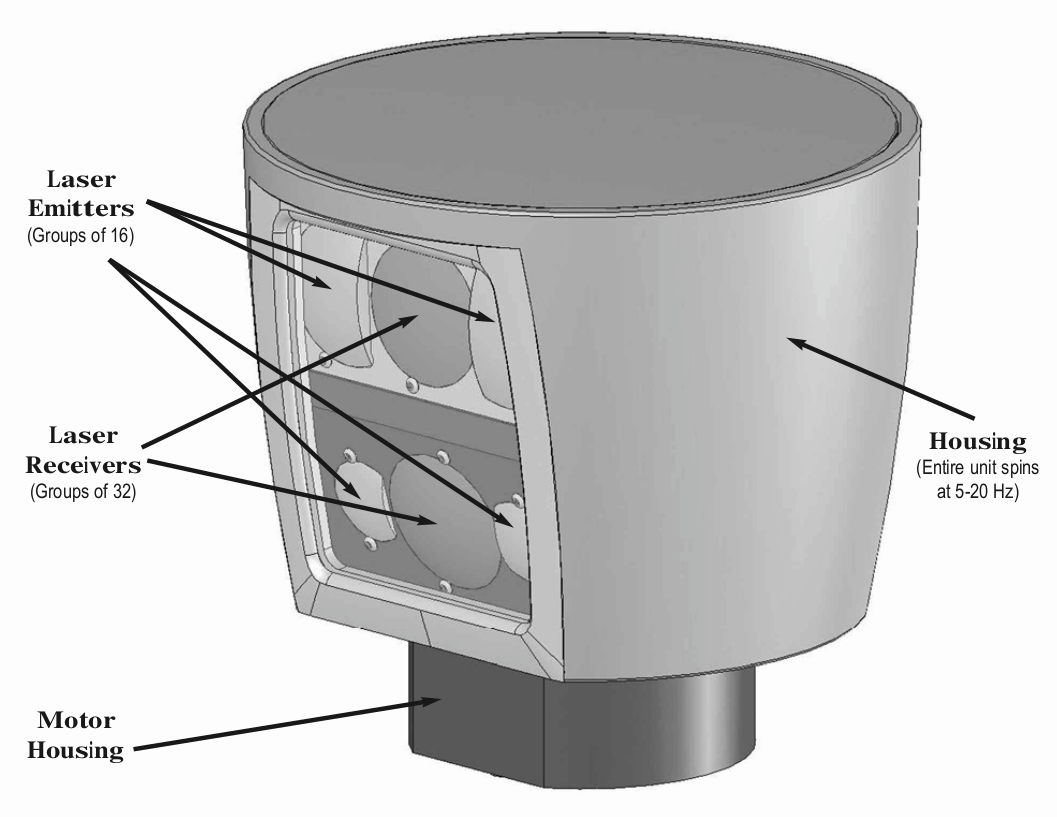
\includegraphics[keepaspectratio,width=0.98\textwidth]{img/lidar.png}
\caption{Scheme of Velodyne HDL-64E LiDAR}
\label{lidarscheme}
\end{figure}

\subsection{Technical details of Velodyne HDL-64E LiDAR}

Velodyne HDL-64E LiDAR produces two types of information for each laser ray -- distance (up to 131 meters) and intensity of the returned ray. The returned intensity depends on the reflectance of the object hit by the laser ray, which in turn depends on the material and the color of the object.

It is possible to operate LiDAR in three modes according to the reported data -- ``strongest'' (the point with the highest intensity is reported), ``last'' (the point with the largest distance is reported, which is useful if one wants to discard partially reflective materials such as glass) or ``both'', meaning that both strongest and last is returned. If they happen to be the same, then the second strongest response is returned as well. If the return mode is either ``strongest'' or ``last'', then the number of returned points is essentially halved since only in ``both'' return mode each laser returns 2 points per firing.

The reported accuracy of the LiDAR is less than two centimeters. It has vertical field of view of 26.8\degree{} with upper block of lasers having vertical resolution of 0.33\degree{} and lower block of lasers having vertical resolution of 0.5\degree. It is able to rotate at various speeds ranging from 300 RPM to 1200 RPM. The data is reported with the same rate regardless of rotation speed, therefore horizontal resolution depends on the current rotational speed. For the speed of 600 RPM (default value~\cite{velomanual}) the horizontal resolution is 0.1728\degree{} and the number of generated points per one rotation of the unit is 133376.
